% !TeX encoding=utf-8
\documentclass[a4paper]{feidippp}
\usepackage[pdftex]{graphicx}
\DeclareGraphicsExtensions{.pdf,.png.,mps.,jpg}
\graphicspath{{figures/}}

\usepackage[utf8]{inputenc}
\usepackage[T1]{fontenc}
\usepackage[slovak]{babel}

\usepackage{lmodern}
\usepackage{graphics}

\usepackage{amsmath,amssymb,amsfonts}

\def\figurename{Obrázok}
\def\tabname{Tabuľka}



%\usepackage[dvips]{graphicx}
%\DeclareGraphicsExtensions{.eps}



%\usepackage[pdftex]{hyperref}   %% tlac !!!
\usepackage[pdftex,colorlinks,citecolor=magenta,bookmarksnumbered,unicode,pdftoolbar=true,pdfmenubar=true,pdfwindowui=true,bookmarksopen=true]{hyperref}

%\usepackage[numbers]{natbib}
\usepackage{natbib} \citestyle{chicago}




\autor{Michaela Horváthová}
\veduci{doc. Ing. Zdeněk Havlice, CSc..}
\konzultant{}
\nazov{Generovanie prototypov z UML}



\datum{30. 4. 2021}



\begin{document}
\bibliographystyle{dcu}



\titulnastrana

\newpage


\tableofcontents



\newpage

\setcounter{page}{1}

\section{Úvod}



\section{	Formulácia úlohy a cieľ práce}


\section{	Analýza súčastného stavu}

 V tejto časti práce bolo naším cieľom  ...

\subsection{MDA}


Model Driven Architecture (MDA), modelom riadená architektúram je špecifikácia konzorcia Object Managment Group (OMG) založená na pevne stanovených štandardoch tejto skupiny a ako štandart bola schválená v roku 2001. Podrobnejšia definícia architektúry bola prijatá v roku 2003 a aktualizovaná v roku 2014 konzorciom OMG. MDA je prechodom všeobecnejšieho modelom riadeného inžinierstva  MDE. MDA definuje pravidlá pre model a architektúry na podporu celého životnéhocyklu vývoja fyzického, organizačného a informačného systému. MDA reprezentuje a podporuje všetky požiadavky pre biznis modelovanie a implementáciu technológií. Pomocou MDA modelov sme schopní lepšie riešiť zložitosti veľkých systémov a intrakcie medzi ľudmi, oraganizáciami,hardvérom a softvérom.
Hlavnou črtou MDA, ktorá nám umožňuje riešiť zložitosti a získať hodnoty z modelov, sú modely  definujúce štruktúru, sémantiku a záznamy modelov pomocou štandardov definovaných v MDA modeloch.
MDA používa na opis systému jazyk UML. MDA je podstate štandardizovaný spôsob ako používať UML ako programovací jazyk. Ak teda hovoríme o MDA, tak sa často hovorí aj o UML, pretože MDA používa UML ako svoj základný modelovací jazyk [1].

MDA charakterizujú pojmy abstrakcia, komunikácia, transformácia a model [1].
Abstrakcia sa používa v MDA v zmysle definovanom v referenčnom modeli overeného distribuvaného spracovanie (ODP) ako potlačenie nepodstatných detailov. Je užitočné charakterizovať modely z hľadiska kritérií použitia, ktoré učujú, čo budepoužité v modeli.  Model, ktorý je založený na špecifickej abstrakcii kritérií , sa často označuje ako model definovaný týmito kritériami.
Komunikácia ako komunikačný prostriedok pomáha tímu nájsť spoločné riešenie pomocou týchto pravidiel:
-	Zabezpečiť zrozumiteľné definície termínov, ktoré pomáhajú pri porozumení danej oblasti.
-	Zebezpečiť základ pre modely – ako majú byť  sémantické údaje zdieľané a spravované.
-	Zabezpečiť knižnicu opakovane použiteľných modelov, slovníkov, pravidiel, procesov alebo architektonických návrhových vzorov.
Transformácia modelov môže byť čiastočné alebo úplne automatizovaná. Automatizácia znižuje náklady a časovú náročnosť na realizáciu projektu, zmey a údržby projektu.
Modely sú nelineárne formy skladajúce sa z prvkov, ktoré sú vzájomne prepojené tak, že vznikajú jednoduché sekvencie, kde každý prvok má väčšinu dva susedné prvky.  Z uvedeného dôvodu sú modely vykreslené pomocou vizuálneho značenia do diagramov, namiesto textu. Model je schematické znázornenie reálneho sveta. Je postavený tak, aby poskytoval lepšie pochopenie vyvíjaného systému. Modely dva zložitých systémov sú vytvorené preto, že tieto systémy nemôžu byť pochopené v plnom rozsahu ako jeden celok. 


\subsection{	Základné pojmy MDA}

Systém  je súbor komponentov a vzťahov medzi týmito časťami, ktoré môžu byť organizované na dosiahnutie cieľa. V MDA termín systém môťe odkazovať na systém pre spracovanie informácii, ale môže byť aplikovaný aj všeobecne. Systém môže zahŕňať čokoľvek – systém hardvéru, softvéru, osôb, atď. Jednou z kľúčových stránok modelovania, ktorá jú odlišuje od implementačných technológií ako je zdrojový kód softvéru, je porozumenie a špecifikácia systému [1].
Modelovací jazyk, každý model musí byť vyjadrený spôsobom, ktorý zobrazuje informácie o systéme medzi zúčastnenými subjektmi, ktoré môžu byť správne interpretované zúčastnenými stranami a podpornými technológiami. Preto je potrebné, aby bol model komunikovaný v jazyku zrozumiteľnom všetkým stranám a technológiam. Dosiahnutie porozumenia znamená, že podmienky, zápisy, syntax, sémantika a pravidlá sú v modeli správne definované,  Pravidlá, štruktúra, pojmy, syntax, sémantika, integrita, poznámky sa používajú na vyjadrenie modelu, ktorý tvorí modelovací jazyk. Známe modelovacie jazyky sú UML, SQL, ER, XML.
Arcitektúra  definuje viac druhov modelov, ktoré majú byť pripravené a použité, a definuje vzťahy medzi jednotlivými modelmi, MDA používa architektúru modelovania, aby realizácia systému bola lacnejšia, jednoduchšia, zrozumiteľná, rýchlejšia a menej riskantná [3].
Architektonické vrstvy  
Je užitočné určiť konkrétne vrstvy architektúry s ohľadom na úroveň abstrakcie.
Kategorizácia konceptu:
Biznis, doménový model – je model skutočných osôb, miest, vecí a zákonov domény. Prípady týchto demén sú skutočné prípady, nie reprezentácia prípadov v informačnom systéme.
Logický systémový model- modely, komponenty systému, ktoré reagujú medzi sebou s ľudmi a organizáciamu v dosahovaní svojich cieľov. 
Implementačné modely – spôsob, akým je konkrétny systém alebo subsystém realizovaná tak, že vykonáva svoje funkcie. Modely implementácie sú viazané na konkrétne realizácie  technológie alebo platformy. 
Transformácie  zaoberajú sa výrobou rôznych modelov založených na transformačnom vzore. Všeobecne platí, že transformácia môže byť použitá na produkovanie jednej reprezentácie z inej, alebo prekročenie úrovne abstrakcie architektonických vrstiev. MDA transformácie poskytujú mechanizmy na transformáciu medzi reprezentáciamia úrovňami abstrakcie alebo architektonických vrstiev.

Platforma je súbor zdrojov, na ktorých je realizovaný systém. Platforma je súbor subsystémov a technológií, ktoré poskytujú ucelený súborfunkcií cez rozhranie a spôsoby používania, ktorých aplikáciu podporovanú platformou možno použiť bez obávz toho, ako sú funkcie poskytované platformou implementované [3].

Pohľad na systém  je technika pre použitie abstraktného súboru architektúry a štrukturovaných pravidiel, na zameranie konkrétnych problémov v rámci systému. Abstrakcia sa používa na označenie procesu, ktorý vytvorí zjednodušený model  [3].


\subsection{Modely MDA}

Táto časť popisuje jednotlivé modely MDA- načo sa používajú, vzťahy medzi nimi a ako medzi sebou súvisia. 

\subsubsection{	CIM}
CIM je výpočtovo nezávislý model, nevykazuje dataily štruktúry systémov. Nazýva sa tiež model domény a využíva slovné zísobu, ktorá je použitá na jeho špecifikáciu.
	Predpokladá sa, že použivané COM nemá vedomosti o modeloch používaných na realizáciu funkcií, ktorých požiadavky sú vyjadrené v CIM. CIM hrá dôležitú úlohu na preklenutie priepasti medzi odborníkom a zákazníkmi. Najčastejšími použivateľmi tohto modelu sú biznis analytici alebo použivatelia systému. 
Požiadavky na systém sú modelované pomocou nezávislého výpočtového modelu CIM, ktorý opisuje situáciu, v ktorej može byť systém použitý. Takýto model sa nazýva aj doménový model alebo biznis model. 

\subsubsection{	PIM}

PIM je model nezávislý na platforme. Vykazuje určitú mieru nezávislosti na platforme, tak aby bola vhodná prepoužitie s rôznymi platformami podobného typu. Veľmi často používaná technika pre dosiahnutie nezávislosti na platforme, je zameranie  sa na systém modelu pre virtuálny stroj technologicky neutrálne.
       
\subsubsection{	PSM}  
PSM, platformovo špecifický model je pohľad na systém z hľadiska konkrétnej platformi, ktorá kombinuje špecifikácie modelu PIM s údajmi, ktoré špecifikujú ako systém používa konkrétny typ platformy. PSM poskytuje súbor technických pojmov, ktoré predstavujú rôzne časti , ktoré tvoria platformu a poskytnuté služby konkrétnej platformy. Tiež stanovuje pre použitie platformy konkrétny model, koncepty predstavujúce rôzny druhy prvkov, ktoré majú byť použité v špecifikácií použitia platformy aplikácií.
	PSM je posledný model specifikácie MDA, ktorý je závislý na platforme. Vzniká transformáciou z platformovo nezávislého modelu PIM s konkrétnym technologickým riešením. Tento model verne odráža štruktúru kódu a preto je vhodný pre implementáciu. Vyskytujú sa v ňom objekty, ktoré úzko súvisa so zvolením tried.


\subsection{Transformácia medzi modelmi }

V tejto kapitole popíšeme modely transformácií, ktoré tvoria kľúčovú časť MDA a prístupy, ktoré sa používajú pre transformáciu modelov.

\subsubsection{		 MDA model transformácie }  
 Je proces konverzie jedného modelu na iný model, v našém prípade transformácia z PIM do PMS, Transformácia predstavuje automatizovanú cestu modelov zainteresovaných strán, ktorej cieľom je aby modely na vysokej úrovni transformovali na spustiteľný IS. Znižuje čas a náklady na výrobu a ľahsšie udržiavanie týchto systémov. Nie všetky modely sú určené pre automatizáciu. Modely musia byť dostatočne podrobné a presné, takže všetky požiadavky pre IS dú vyjadrené v modeloch.
MDA slúži k oddeleniu rizika medzi požiadavkami na obchodný systém a technológiu, ktorá ho implementuje. Toto oddelenie obáv je dosiahnuté použitím vzorcov definovaných ako biznis model zameraný na transformáciu a technologické riešenie. 
Obrázok 1. znázorňuje vzor MDA, ktorým je PIM trensformovaná do PMS.




\begin{figure}[!ht]
\centering 
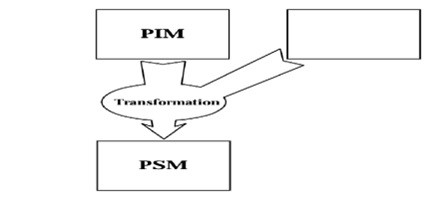
\includegraphics[width=0.5\textwidth]{dp1.jpg}
\caption{ Transformácia  z PIM do PMS}\label{o:1}
\end{figure}


\subsubsection{	Transformácia metamodelu }

Model je pripravený používať platformu nezávislú na jazyku určenú metamodelom. Platforma je vyberaná autorom modelu. Špecifikácia transformácie pre túto platformu je k dispozícií, alebo sa pripravuje. Špecifikácia transformácie sa používa vtedy, ak sa vykonáva mapovanie medzi modelmi. Pomocou mapovania sa uskutoční transformácia z PIM do PMS, príklad je uvedený na obrázku 2. [1].

\begin{figure}[!ht]
\centering 
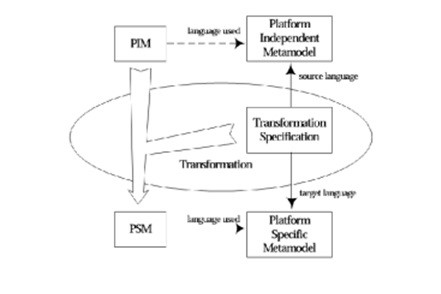
\includegraphics[width=0.5\textwidth]{dp2.jpg}
\caption{ Transformácia metamodelom}\label{o:1}
\end{figure}



\subsubsection{	Transformačný model } 


Model používa typy nezávislé na platforme špecifikované v modeli. Tieto typy môžu byť súčasťou softvéru. Prvky v PIM sú podtypy nezávislých typov platformy. Platforma je vybraná a špecifikácia transformácie pre túto platformu je k dispozícii. Táto transformácia špecifikujem mapovanie medzi typmi nezávislých na platforme a typmi závislými na platforme. Prvky v PSM sú podtypy špecifických typov platformy.

\begin{figure}[!ht]
\centering 
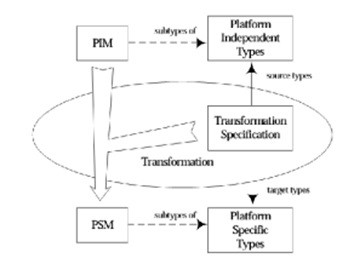
\includegraphics[width=0.5\textwidth]{dp3.jpg}
\caption{ Transformačný model}\label{o:1}
\end{figure}






\subsection{	Charakteristika UML jazyka}


Diagramy UML sú výstupom Unified Modeling Language. Je to obrazové znázornenie tried, objektov a vzťahov medzi nimi. Diagram UML je model, ktorý popisuje časť systému. Používa sa na definovanie funkčnosti alebo návrhu systému. Diagram musí byť jasný a stručný, aby ho divák ľahko pochopil. UML má aplikácie presahujúce vývoj softvéru, napríklad tok procesov vo výrobe. Je to analogické s plánmi používanými v iných oblastiach a pozostáva z rôznych typov diagramov. V súhrne UML diagramy popisujú hranice, štruktúru a chovanie systému a objektov v ňom. UML nie je programovací jazyk, ale existujú nástroje, ktoré možno použiť na generovanie kódu v rôznych jazykoch pomocou diagramov UML. UML má priamy vzťah s objektovo orientovanou analýzou a návrhom. V informatike existuje veľa paradigiem alebo modelov na riešenie problémov, čo je štúdium algoritmov a údajov. Existujú štyri kategórie modelov riešenia problémov: imperatívne, funkčné, deklaratívne a objektovo orientované jazyky (OOP). V objektovo orientovaných jazykoch sú algoritmy vyjadrené definovaním „objektov“ a ich vzájomnou interakciou. S týmito objektmi je potrebné manipulovať a existujú v skutočnom svete. Môžu to byť budovy, miniaplikácie na pracovnej ploche alebo ľudia.  
Objektovo orientované jazyky dominujú v programovacom svete, pretože modelujú objekty v reálnom svete. UML je kombináciou niekoľkých objektovo orientovaných notácií: Objektovo orientovaný dizajn, Technika modelovania objektov a Objektovo orientované softvérové inžinierstvo. UML využíva silné stránky týchto troch prístupov na predstavenie konzistentnejšej metodiky, ktorá sa ľahšie používa. UML predstavuje najlepšie postupy pre vytváranie a dokumentovanie rôznych aspektov modelovania softvéru a obchodných systémov [7]. 



\begin{figure}[!ht]
\centering 
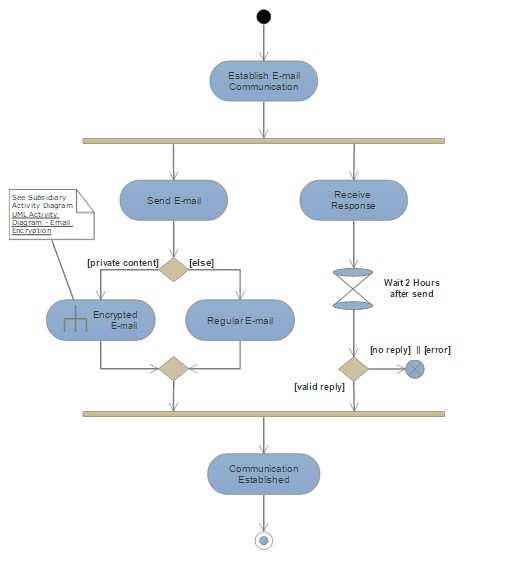
\includegraphics[width=0.5\textwidth]{dp4.jpg}
\end{figure}


Diagramy UML sú rozdelené do troch rôznych kategórií, ako napríklad: [5].

\begin{itemize}
  \item Štrukturálny diagram,
  \item Behaviorálny diagram, 
  \item Interakčný diagram.
\end{itemize}


\textbf {Strukturálne diagramy}

Štrukturálne diagramy sa používajú na predstavenie statického pohľadu na systém. Predstavuje súčasť systému, ktorá tvorí štruktúru systému. Štrukturálny diagram zobrazuje rôzne objekty v systéme.
Nasledujú rôzne štrukturálne diagramy v UML:


\begin{itemize}
  \item Diagram triedy,
  \item Objektový diagram, 
  \item Schéma balenia,
  \item Schéma komponentov,
  \item Schéma nasadenia.
  
\end{itemize}

\textbf {Behaviorálne diagramy}

Akýkoľvek systém v reálnom svete môže byť reprezentovaný buď v statickej alebo dynamickej podobe. Systém sa považuje za kompletný, ak je vyjadrený statickým aj dynamickým spôsobom. Diagram správania predstavuje fungovanie systému.
Diagramy UML, ktoré sa zaoberajú statickou časťou systému, sa nazývajú štruktúrne diagramy. Diagramy UML, ktoré sa zaoberajú pohyblivými alebo dynamickými časťami systému, sa nazývajú diagramy správania [7].
Nasledujú rôzne diagramy správania v UML:

\begin{itemize}
  \item Schéma činnosti,
  \item Použite diagram prípadov, 
  \item Schéma stavového automatu.
  
\end{itemize}



\textbf {Interakčné diagramy}

Interakčný diagram nie je nič iné ako podmnožina behaviorálnych diagramov. Používa sa na vizualizáciu toku medzi rôznymi prvkami systému v prípade použitia. Interakčné diagramy sa používajú na znázornenie interakcie medzi dvoma entitami a spôsobu toku údajov v nich.

\textbf {Nasledujú rôzne interakčné diagramy v UML:}


\begin{itemize}
  \item Časový diagram,
  \item Sekvenčný diagram, 
  \item Schéma spolupráce.
  
\end{itemize}


\subsubsection{Nástroje UML}

Na trhu existuje veľa nástrojov na generovanie UML diagramov. Niektoré sú založené na počítači, zatiaľ čo iné sa dajú používať online. Nasleduje prehľadný zoznam nástrojov, ktoré možno použiť na vytvorenie modelov UML:


\begin{itemize}
  \item Argo UML,
  \item Dia, 
  \item Vizuálna paradigma,
  \item U-model,
  \item Hviezdička UML,
  \item 	UML laboratórium.
  
\end{itemize}

\subsubsection{Typy diagramov UML}

Súčasné štandardy UML požadujú 13 rôznych typov diagramov: trieda, aktivita, objekt, prípad použitia, postupnosť, balík, stav, komponent, komunikácia, zložená štruktúra, prehľad interakcií, načasovanie a nasadenie.
Tieto diagramy sú usporiadané do dvoch samostatných skupín: štrukturálne diagramy a diagramy správania alebo interakcie [5].

\textbf{Štrukturálne diagramy UML:}

\begin{itemize}
\item	Diagram triedy,			
\item Sekvenčný diagram,
\item Použite diagram prípadov,
\item Stavový diagram,
\item Komunikačný diagram,
\item Prehľadný prehľad interakcií,
\item Časový diagram.
  
  \end{itemize}
  \begin{itemize}
      
  
\item Schéma balenia,
\item Objektový diagram,
\item Schéma komponentov,
\item Zložený štruktúrny diagram,
\item Schéma nasadenia.

\end{itemize}	


\textbf{ Diagram tried}
Tieto diagramy sú chrbticou takmer každej objektovo orientovanej metódy vrátane UML. Opisujú statickú štruktúru systému[9]. 
	
\textbf{Schéma}
Schémy balíka sú podmnožinou diagramov tried, vývojári ich však niekedy považujú za samostatnú techniku. Schémy balíkov organizujú prvky systému do príbuzných skupín, aby sa minimalizovali závislosti medzi balíkmi [9]. 



\textbf {Objektový diagram}

Objektový diagram popisuje statickú štruktúru systému v konkrétnom čase. Môžu byť použité na testovanie presnosti diagramov tried.

\textbf {Diagram prípadov použitia}

Modelujú funkčnosť systému pomocou aktérov a prípadov použitia.



\textbf {Diagram aktivít}

 	Tieto diagramy ilustrujú dynamickú povahu systému modelovaním toku kontroly od aktivity k činnosti. Aktivita predstavuje operáciu na nejakej triede v systéme, ktorá má za následok zmenu stavu systému. Diagramy aktivít sa zvyčajne používajú na modelovanie pracovných tokov alebo obchodných procesov a internej prevádzky.
  
\textbf {Sekvenčný diagram}

Sekvenčné diagramy popisujú interakcie medzi triedami z hľadiska výmeny správ v priebehu času.

\textbf {Časový diagram}

Časový diagram je typ behaviorálneho alebo interakčného diagramu UML, ktorý sa zameriava na procesy, ktoré prebiehajú počas konkrétneho časového obdobia. Sú špeciálnou inštanciou sekvenčného diagramu, až na to, že sa ukazuje, že čas sa zvyšuje zľava doprava namiesto zhora nadol.

\textbf {Komunikačný diagram}

Komunikačné diagramy modelujú postupné interakcie medzi objektmi. Opisujú statickú štruktúru aj dynamické správanie systému. V mnohých ohľadoch je komunikačný diagram zjednodušenou verziou diagramu spolupráce zavedeného v UML 2.0.



\textbf {Stavový diagram }

Stavové diagramy, teraz známe ako stavové automaty a stavové diagramy, popisujú dynamické správanie systému v reakcii na vonkajšie podnety. Stavové diagramy sú obzvlášť užitočné pri modelovaní reaktívnych objektov, ktorých stavy sú spúšťané konkrétnymi udalosťami.


\subsubsection {Symboly UML diagramu }


Existuje veľa rôznych typov diagramov UML a každá z nich má mierne odlišnú sadu symbolov.
Diagramy tried sú možno jedným z najbežnejších použitých diagramov UML a symboly diagramov tried sa sústreďujú okolo definovania atribútov triedy. Napríklad existujú symboly pre aktívne triedy a rozhrania. Symbol triedy možno tiež rozdeliť tak, aby zobrazoval operácie, atribúty a zodpovednosti triedy.
Viditeľnosť všetkých členov triedy je označená poznámkami.


\begin{figure}[!ht]
\centering 
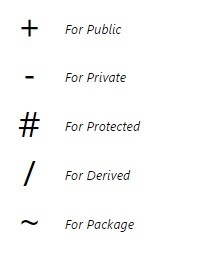
\includegraphics[width=0.5\textwidth]{dp.jpg}

\end{figure}

\textbf{Riadky sú tiež dôležitými symbolmi označujúcimi vzťahy medzi komponentmi. Zovšeobecnenie a dedenie sú označené prázdnymi šípkami. Zloženie je zobrazené s vyplneným diamantom. Agregácia je zobrazená s prázdnym kosoštvorcom. Závislosti sú označené prerušovanou čiarou so šípkou. Použitie << >> vám umožňuje označiť vlastnosti tejto závislosti. Násobnosť sa zvyčajne zobrazuje s číslom na jednom konci šípky a znakom * na druhom konci [9].}


\begin{figure}[!ht]
\centering 
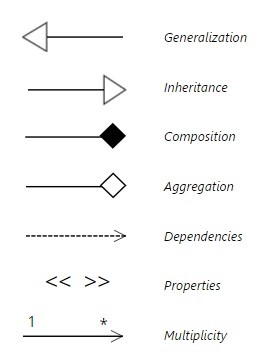
\includegraphics[width=0.5\textwidth]{dp5.jpg}
\caption{ Transformačný model}\label{o:1}
\end{figure}

\textbf{Schémy balíkov obsahujú symboly definujúce balík, ktorý vyzerá ako priečinok.}

\begin{figure}[!ht]
\centering 
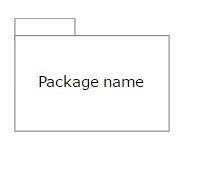
\includegraphics[width=0.5\textwidth]{dp6.jpg}
\end{figure}

Diagramy aktivít obsahujú symboly pre aktivity, stavy, vrátane samostatných symbolov pre počiatočný stav a konečný stav. Tok riadenia je zvyčajne zobrazený šípkou a tok objektov zobrazený prerušovanou šípkou.

\begin{figure}[!ht]
\centering 
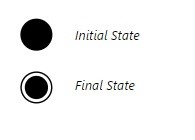
\includegraphics[width=0.5\textwidth]{dp7.jpg}
\end{figure}

\textbf{Schémy prípadov použitia majú symboly pre hercov a prípady použitia.}

\subsubsection{Účel UML podľa OMG}

Poskytuje  systémovým architektom, softvérovým inžinierom a vývojárom softvéru s nástrojmi na analýzu, návrh a implementáciu softvérových systémov, ako aj na modelovanie obchodných a podobných procesov.
Umoňuje posilnenie stavu v odbore umožnením interoperability nástroja vizuálneho modelovania objektov. Taktiež slúži na umožnenie zmysluplnej výmeny modelových informácií medzi nástrojmi je však potrebná dohoda o sémantike a notácii.


\textbf{UML musí spĺňať nasledujúce požiadavky:}

-	Stanovenie formálnej definície spoločného meta-modelu založeného na metaobjektových zariadeniach (MOF), ktorý špecifikuje abstraktnú syntax UML. Abstraktná syntax definuje množinu konceptov modelovania UML, ich atribúty a ich vzťahy, ako aj pravidlá kombinácie týchto konceptov na konštrukciu čiastkových alebo úplných modelov UML.

-	Poskytnutie podrobného vysvetlenia sémantiky každého konceptu modelovania UML. Sémantika definuje technologicky nezávislým spôsobom, ako majú byť koncepty UML realizované počítačmi.

-  Špecifikácia ľudsky čitateľných prvkov notácie na reprezentáciu jednotlivých koncepcií modelovania UML, ako aj pravidlá ich kombinovania do rôznych typov diagramov zodpovedajúcich rôznym aspektom modelovaných systémov.

-  Definovanie spôsobov, ako je možné dosiahnuť, aby boli nástroje UML v súlade s touto špecifikáciou. Toto je podporované (v samostatnej špecifikácii) špecifikáciou zodpovedajúcich formátov výmeny modelov (XMI) založených na XML, ktorú je potrebné realizovať pomocou kompatibilných nástrojov.

\subsubsection{Meant by UML}

UML znamená Unified Modeling Language. UML 2.0 pomohla rozšíriť pôvodnú špecifikáciu UML tak, aby pokrývala väčšiu časť úsilia pri vývoji softvéru vrátane agilných postupov [4].
Vylepšená integrácia medzi štrukturálnymi modelmi, ako sú diagramy tried, a modelmi správania, ako sú diagramy aktivít.
Bola pridaná možnosť definovať hierarchiu a rozložiť softvérový systém na komponenty a čiastkové komponenty.
Pôvodný UML špecifikoval deväť diagramov; UML 2.x zvyšuje toto číslo na 13. Štyri nové diagramy sa nazývajú: komunikačný diagram, diagram zloženej štruktúry, prehľadný prehľad interakcií a časovací diagram. Tiež premenovala diagramy stavových diagramov na diagramy stavových strojov, známe tiež ako stavové diagramy.



\subsubsection{UML a dátové modelovanie}

UML a dátové modelovanie UML je populárny medzi programátormi, vývojári databáz ho však všeobecne nepoužívajú. Jedným z dôvodov je jednoducho to, že sa tvorcovia UML nesústredili na databázy. Napriek tomu je UML efektívny pre koncepčné dátové modelovanie na vysokej úrovni a dá sa použiť v rôznych typoch UML diagramov. 

\subsubsection{Príklady diagramu UML}

Najlepší spôsob, ako porozumieť UML, je pozrieť sa na niektoré príklady diagramov UML[9]. 


\begin{figure}[!ht]
\centering 
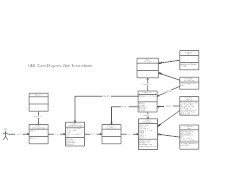
\includegraphics[width=0.5\textwidth]{dp8.jpg}
\caption{Schéma činnosti - spracovanie objednávky}
\end{figure}


\begin{figure}[!ht]
\centering 
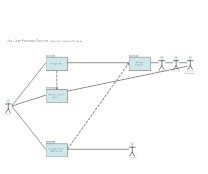
\includegraphics[width=0.5\textwidth]{dp9.jpg}
\caption{Diagram triedy - webové transakciey}
\end{figure}

\subsubsection{Možnosti využitia UML jazyka v rámci návrhu prototypov}
\subsubsection{ Metodológia pre vytvorenie generátora prototypov z UML diagramov}

\section{	Modely UML v MDA}

UML modely sú deklaratívne modely ako IDL, Jana, Microsoft- rozhranie.
Myšlienkou MDA je transformovať deklaratívne UML modely pomocou vzorov v MDA na kodel s konkrétnym tozhraním. UML modely sa líšia od iných deklaratívnych modelov v nasledujúcich dôležitých aspektoch:

\begin{enumerate}
  \item 	UML definuje základné koncepty modelovania a týn posiľňuje MDA, 
  \item UML modely môžu byť vyjadrené textovo aj graficky, 
  \item .	UML modely sú sémanticky oveľa bohatšie ako jazyk deklaratívnych modelov, ktoré môžu byť vyjadrené syntaxou, ale obsahujú niektoré obmedzenia na používanie a správanie:. 
\end{enumerate}


-	Nemenné obmedzenie atribútov,
-	Dvojica predpokladov a podmienok pre špecifikovanie operácií,
-	Jednoduchá hodnota parametra nesmie byť nula,
-	Operácia má vedlajsoe účinky,
-	Podtypy nejakého super typu sú disjunktné, alebo tvoria oddiel

\section{Vytvorenie množiny vhodných UML modelov}
/Bankomat
Knižnica - požičanie knihy, vrátenie atď.
Cestovná kancelária
Odpadové hospodárstvo/

\section{	Návrh generátora prototypov}
/UI generátor prototypov
Transformačné pravidlá
Transformačný algoritmus
Príklad transformácie/

\section{Implementácia generátora na konkrétne UML modely}
\section{Zhodnotenie vytvorených prototypov}
\section{	Zhodnotenie vytvorených prototypov}
\section{Testovanie nástroja}



\addcontentsline{toc}{section}{\numberline{}Zoznam obrázkov}
\listoffigures

\addcontentsline{toc}{section}{\numberline{}Zoznam tabuliek}
\listoftables


\def\refname{Zoznam použitej literatúry}
\addcontentsline{toc}{section}{\numberline{}Zoznam použitej literatúry}

\begin{thebibliography}{999}
\harvarditem{Gonda}{2001}{gonda} [1].Model Driven Architecture[online]. [cit. 2004-02-02]. Dostupné z: \emph{https://martinfowler.com/bliki/ModelDrivenArchitecture.html}

\harvarditem{Gonda}{2001}{gonda}
[2].Service oriented architecture Modeling Language  [online]. [cit. 2012-05]. \emph{Dostupné z: https://www.omg.org/spec/SoaML/1.0.1/PDF} Bratislava : Elita, 2001, 

\harvarditem{Jadr. fyz. a~tech.}{1985}{slovnik}
[3].	Model Driven Architecture  [online]. [cit. 2004-02-02]. \emph{https://www.omg.org/mda/} 

\harvarditem{Katuščák}{1998}{kat}
[4].	What is UML [online]. [cit. 2013]. \emph{Dostupné z: https://www.visual-paradigm.com/guide/uml-unified-modeling-language/what-is-uml/} 

%\harvarditem{Sýkora a~i.}{1980}{sykora}
%SÝKORA, F. a~iní. 1980. \emph{Telesná výchova a~šport.} 1.~vyd. Bratislava : SPN, 1980. 35 s. ISBN 80-8046-020-5

\harvarditem{Lamoš a~Potocký}{1989}{lamos}
UML diagram  [online]. [cit. 2016]. \emph{]. Dostupné z:  https://www.smartdraw.com/uml-diagram/} 

\harvarditem{Sýkora a~i.}{1980}{sykora}
[6].What is Unified Modeling Language [online].  \emph{https://www.lucidchart.com/pages/what-is-UML-unified-modeling-language} 

\harvarditem{Lamoš a~Potocký}{1989}{lamos}
[7].What is UML [online]. [cit. 2013]. . \emph{Dostupné z: https://www.uml.org/what-is-uml.htm} 

\harvarditem{Lamoš a~Potocký}{1989}{lamos}
[7].What is UML [online]. [cit. 2013]. . \emph{Dostupné z: https://www.uml.org/what-is-uml.htm} 

\harvarditem{Lamoš a~Potocký}{1989}{lamos}
[8].What do their creators think about UML [online].  \emph{https://modeling-languages.com/uml-opinions-creators/} 

\harvarditem{Lamoš a~Potocký}{1989}{lamos}
[9].A Comprehensive Guide to 14 Types of UML Diagram  [online].[cit. 2020-02-05].   \emph{Dostupné z: https://warren2lynch.medium.com/a-comprehensive-guide-to-14-types-of-uml-diagram-affcc688377e} 

\harvarditem{Lamoš a~Potocký}{1989}{lamos}
[10].UML Diagrams guide [online]. [cit. 2013]. \emph{ Dostupné z: https://cacoo.com/resources/uml-diagrams-guide/} 

\harvarditem{Lamoš a~Potocký}{1989}{lamos}
[11].UML Diagrams [online]. [cit. 2013]. \emph{ Dostupné z: [11].	https://www.buildingsmart.org/wp-content/uploads/2020/06/IR-CS-WP2-UML_Model_Report_Part-1_.pdf

} 

\end{thebibliography}


\end{document}


